\section{Functional Requirements Specification}
\label{sec:functional_requirements}

\subsection{Methodology \& MoSCoW Prioritisation}
\label{subsec:moscow}

To rigorously control project scope, guarantee $100\%$ implementation feasibility in Assignment 02, and maintain direct alignment with the empirical user elicitation findings from Section~\ref{sec:problem_analysis}, all functional requirements of the \textbf{Naomi} platform are classified using the \textbf{MoSCoW Prioritisation Framework}:
\begin{itemize}
    \item \badgeMust{} \textbf{(Core Acceptance Baseline):} Non-negotiable functional capabilities required for the system to operate end-to-end; $100\%$ of Must-Have requirements must pass acceptance verification in Assignment 02.
    \item \badgeShould{} \textbf{(High-Value Experience Enhancers):} Important features that elevate user experience, resilience, and personalisation to a production-grade standard ($90\text{--}100\%$ target rubric band).
    \item \badgeCould{} \textbf{(Innovative Smart Extensions):} Advanced AI/computer-vision capabilities (Visual Search and In-Place AI Chapter Translation) implemented as modular prototypes without compromising core stability.
    \item \badgeWont{} \textbf{(Explicitly Excluded Scope):} Features intentionally omitted from the project boundary to preserve our non-commercial, ad-free, distraction-free \textit{Content-First} philosophy.
\end{itemize}

Table~\ref{tab:fr_matrix} defines the complete catalogue of 17 Functional Requirements (\texttt{FR-00} through \texttt{FR-16}).

\begin{small}
\renewcommand{\arraystretch}{1.28}
\begin{longtable}{C{1.4cm} L{3.6cm} C{2.6cm} p{7.1cm}}
\caption{Master Functional Requirements Matrix with MoSCoW prioritisation (\texttt{FR-00} to \texttt{FR-16}).}
\label{tab:fr_matrix} \\
\toprule
\rowcolor{tablehead}
\textbf{FR ID} & \textbf{Requirement Name} & \textbf{MoSCoW} & \textbf{System Business Capability Description} \\
\midrule
\endfirsthead
\multicolumn{4}{c}{{\bfseries \tablename\ \thetable{} -- continued from previous page}} \\
\toprule
\rowcolor{tablehead}
\textbf{FR ID} & \textbf{Requirement Name} & \textbf{MoSCoW} & \textbf{System Business Capability Description} \\
\midrule
\endhead
\midrule \multicolumn{4}{r}{{Continued on next page}} \\ \bottomrule
\endfoot
\bottomrule
\endlastfoot

\textbf{FR-00} & \textbf{User Account Authentication} & \badgeMust & Enables users to register, sign in, and request password recovery via Email/Password (\texttt{Supabase Auth}). Persists encrypted JWT sessions in hardware-backed storage. Excludes third-party OAuth social logins to maintain provider independence. \\
\rowcolor{tablerow}
\textbf{FR-01} & \textbf{Comic Discovery \& Search (MangaDex API)} & \badgeMust & Searches comics by title or author keyword; organises horizontal discovery rows by \textit{Trending} and \textit{Genre} (\textit{Fantasy, Action}, etc.); supports expanding any row into a full paginated grid (\texttt{S03b}). \\
\textbf{FR-02} & \textbf{Full-Screen Distraction-Free Reader} & \badgeMust & Renders chapter pages across $100\%$ of the viewport; provides a single translucent top icon toolbar for chapter navigation and a 1-tap \textit{Focus Mode} that hides all UI chrome. \\
\rowcolor{tablerow}
\textbf{FR-03} & \textbf{Flexible Dual Reading Mode Toggle} & \badgeMust & Allows instant in-reader switching between continuous vertical scrolling (\textit{Webtoon long-strip mode}) and horizontal paginated flipping (\textit{traditional Manga mode}). \\
\textbf{FR-04} & \textbf{Auto-Save Progress \& Instant Resume} & \badgeMust & Automatically records the exact chapter and page number (\texttt{last\_page\_read}) into local SQLite and synchronises to Supabase Cloud; surfaces a 1-tap \textit{Continue} hero card on the Home screen (\texttt{S02}). \\
\rowcolor{tablerow}
\textbf{FR-05} & \textbf{Genre-Matched Instrumental Ambient Audio} & \badgeMust & Automatically recommends and streams instrumental background audio tracks matching the primary genre of the active comic to foster an immersive, relaxing reading atmosphere. \\
\textbf{FR-06} & \textbf{Offline Chapter Download} & \badgeMust & Downloads all page image assets of selected chapters to sandboxed device storage for offline reading; displays real-time percentage and byte progress (\texttt{S11}). \\
\rowcolor{tablerow}
\textbf{FR-07} & \textbf{Personal Library Management} & \badgeMust & Provides a dedicated two-button Library hub (\texttt{S07}) separating \textit{Favorites} (cloud-synced bookmarked series) and \textit{Offline Reading} (locally saved chapters with storage footprint metrics). \\
\textbf{FR-08} & \textbf{Consolidated Home Feed \& Recommendations} & \badgeShould & Presents a streamlined three-block Home screen (\texttt{S02}): (1) \textit{Continue Reading} hero card, (2) \textit{Recent} horizontal carousel, and (3) \textit{Recommended} horizontal carousel based on genres. \\
\rowcolor{tablerow}
\textbf{FR-09} & \textbf{Minimalist Audio Sheet Controls} & \badgeShould & Provides a clean bottom sheet (\texttt{S06}) with Play/Pause toggle, continuous volume slider, and track selection among genre-matched instrumentals; auto-pauses on phone calls or app backgrounding. \\
\textbf{FR-10} & \textbf{Comic Detail View \& Quick Chapter Actions} & \badgeShould & Displays complete comic metadata (cover, author, rating, genres, synopsis), four primary action buttons (\textit{Read First, Read Latest, Favorite, Download}), and the full chapter list (\texttt{S04}). \\
\rowcolor{tablerow}
\textbf{FR-11} & \textbf{Smart Visual Search via System Photo Picker} & \badgeCould & Allows users to select a comic panel screenshot via the OS \texttt{System Photo Picker} (requiring zero storage permissions) to identify the matching series (\texttt{S03}). \\
\textbf{FR-12} & \textbf{In-Place AI Chapter Translation} & \badgeCould & Integrates an on-demand AI translation action (\texttt{S05} Icon $\star$) that translates dialogue text across the currently open chapter into the user's target language. \\
\rowcolor{tablerow}
\textbf{FR-13} & \textbf{Offline Network Loss Fallback} & \badgeShould & Detects loss of Internet connectivity when opening an uncached chapter, displays a friendly offline error state (\texttt{S09}), and provides a direct CTA button routing to the Offline Library (\texttt{S07}). \\
\textbf{FR-14} & \textbf{User Profile \& System Settings Customisation} & \badgeShould & Manages user profile details, appearance theme (\textit{System / Light / Dark}), UI language (\textit{English / Vietnamese}), disk cache inspection/clearing, notification toggles, and sign-out (\texttt{S08}). \\
\rowcolor{tablerow}
\textbf{FR-15} & \textbf{In-App Purchases (IAP) \& Virtual Coins} & \badgeWont & Explicitly excluded to uphold a $100\%$ non-commercial, paywall-free reading environment. \\
\textbf{FR-16} & \textbf{In-App Social Feed \& 1-on-1 Direct Messaging} & \badgeWont & Explicitly excluded to eliminate social clutter and keep architectural complexity focused on reading performance. \\
\end{longtable}
\end{small}

\subsection{System Use Case Diagram}
\label{subsec:use_case_diagram}

Figure~\ref{fig:use_case_diagram} illustrates the UML 2.5 Use Case Diagram modelling all interactions between the primary human actor (\textbf{Reader}), the nine core use cases (\texttt{UC-00} to \texttt{UC-08}) inside the \textbf{Naomi Mobile Application} boundary, and the two external system actors (\textbf{Supabase Backend} and \textbf{MangaDex REST API}). Mandatory sub-flows are linked via \texttt{<<include>>} dependencies (\texttt{UC-03} includes \texttt{UC-05}), while optional contextual enrichments are modelled via \texttt{<<extend>>} dependencies (\texttt{UC-04} extends \texttt{UC-03}; \texttt{UC-02} extends \texttt{UC-01}; \texttt{UC-06} extends \texttt{UC-07}).

\begin{figure}[H]
    \centering
    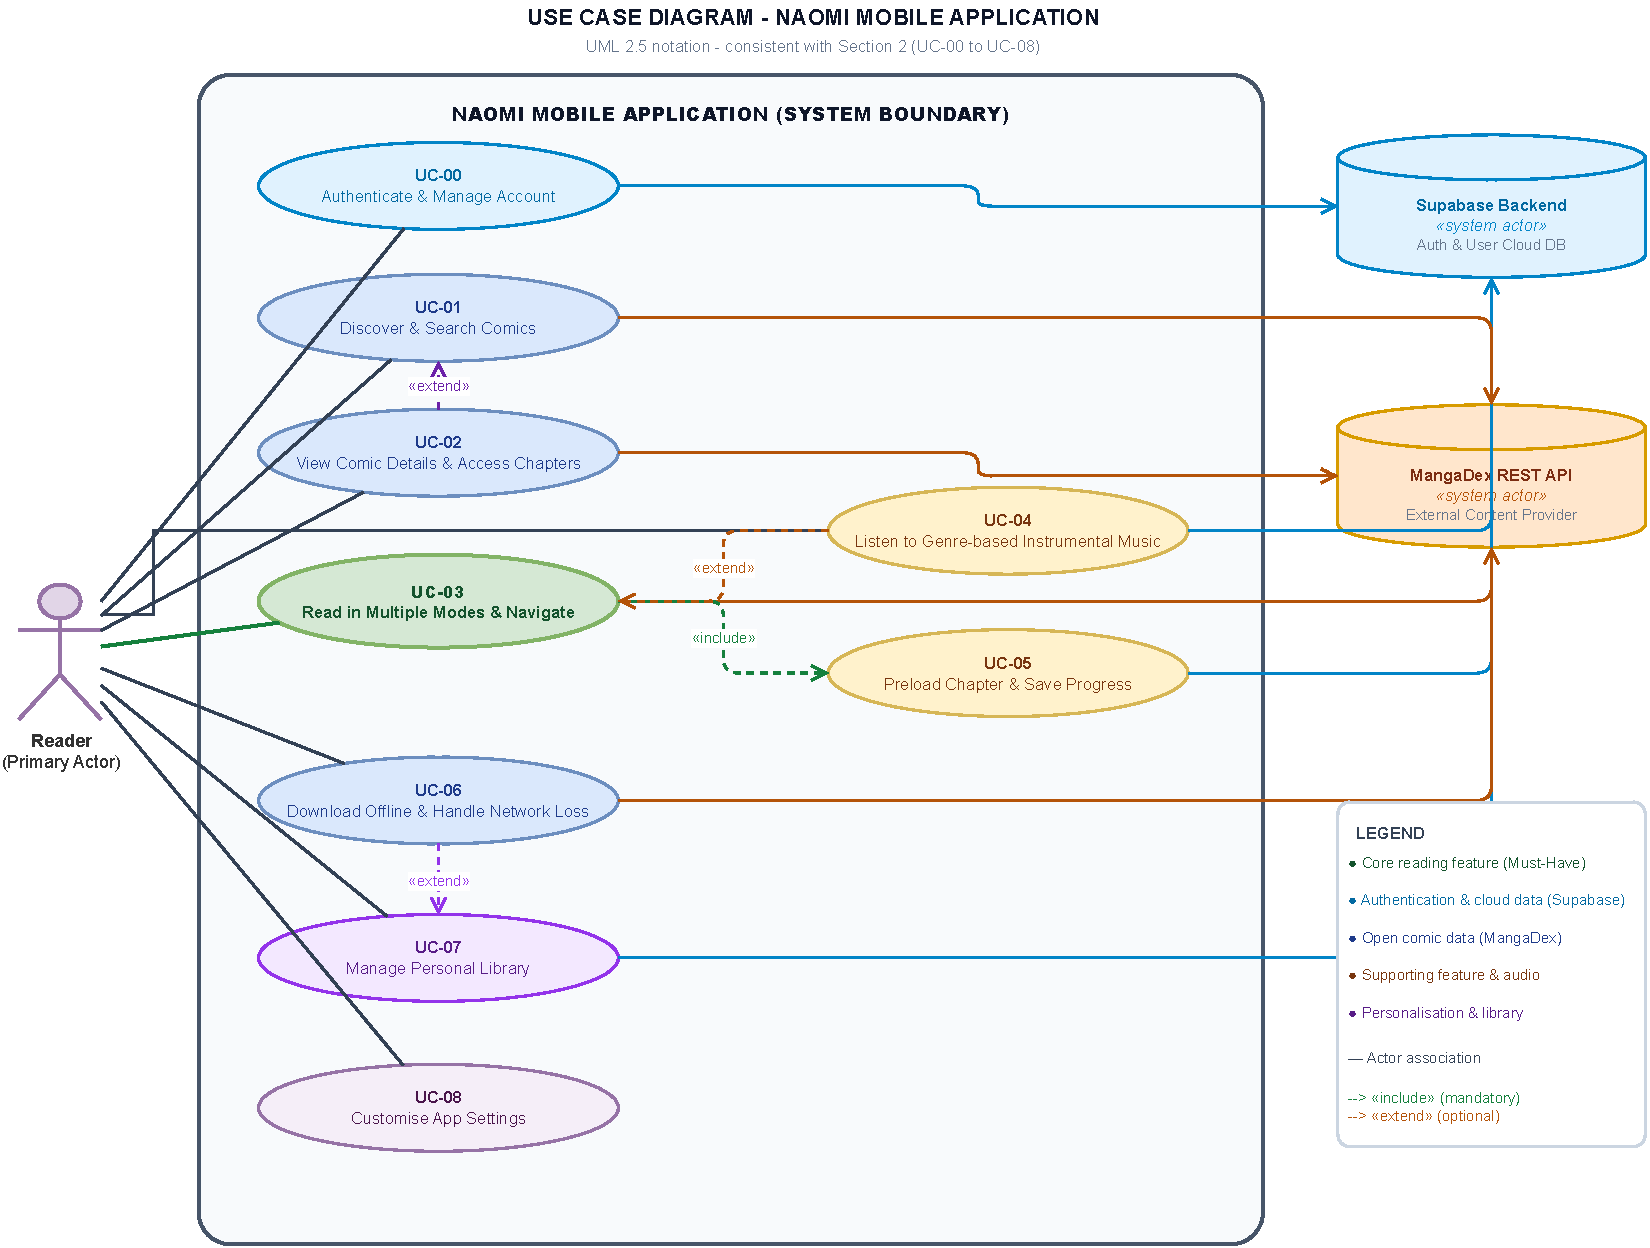
\includegraphics[width=0.98\textwidth]{figures/diagrams/use_case_diagram.pdf}
    \caption{UML 2.5 System Use Case Diagram for the Naomi Mobile Application (\texttt{UC-00} to \texttt{UC-08}).}
    \label{fig:use_case_diagram}
\end{figure}

\subsection{Detailed Use Case Specifications}
\label{subsec:use_case_specs}

Table~\ref{tab:uc_summary} summarises the scope of the nine system use cases, followed by their complete structured specifications (Actors, Preconditions, Postconditions, Main Success Scenario, Alternative Flows, and Exception Flows).

\begin{table}[H]
\centering
\caption{Overview of the nine system Use Cases (\texttt{UC-00} to \texttt{UC-08}).}
\label{tab:uc_summary}
\footnotesize
\renewcommand{\arraystretch}{1.22}
\begin{tabularx}{\textwidth}{C{1.4cm} L{4.6cm} C{2.3cm} Y}
\toprule
\rowcolor{tablehead}
\textbf{UC ID} & \textbf{Use Case Name} & \textbf{Primary Actor} & \textbf{Business Goal} \\
\midrule
\textbf{UC-00} & Authenticate \& Manage Account & Reader & Sign up, sign in, or reset password via Email/Password; persist encrypted JWT session via Supabase Auth. \\
\rowcolor{tablerow}
\textbf{UC-01} & Discover \& Search Comics & Reader & Search comics by keyword, browse \textit{Trending} and \textit{Genre} rows, expand full lists, or search by image (\texttt{FR-11}). \\
\textbf{UC-02} & View Comic Details \& Access Chapters & Reader & Inspect comic metadata, trigger \textit{Read First / Read Latest}, bookmark to \textit{Favorites}, or initiate chapter downloads. \\
\rowcolor{tablerow}
\textbf{UC-03} & Read in Multiple Modes \& Navigate & Reader & Read full-screen pages, toggle Vertical Webtoon $\leftrightarrow$ Horizontal Manga, switch chapters, and activate \textit{Focus Mode}. \\
\textbf{UC-04} & Listen to Genre-Based Instrumental Music & Reader & Stream instrumental ambient tracks matched to the comic's genre; control playback, volume, and track selection. \\
\rowcolor{tablerow}
\textbf{UC-05} & Preload Chapter \& Save Progress & System / Reader & Pre-buffer $100\%$ of chapter pages before opening the reader (\texttt{S10}); continuously persist page progress to SQLite \& Cloud. \\
\textbf{UC-06} & Download Offline \& Handle Network Loss & Reader & Download chapter page assets into sandboxed local storage (\texttt{S11}); route gracefully to Offline Library on network loss (\texttt{S09}). \\
\rowcolor{tablerow}
\textbf{UC-07} & Manage Personal Library & Reader & Access and manage the two-button Personal Library (\texttt{S07}): cloud-synced \textit{Favorites} and local \textit{Offline Reading}. \\
\textbf{UC-08} & Customise App Settings & Reader & Configure appearance theme (\textit{System/Light/Dark}), UI language, disk cache cleanup, notifications, and sign-out (\texttt{S08}). \\
\bottomrule
\end{tabularx}
\end{table}

\subsubsection{UC-00: Authenticate \& Manage User Account}
\begin{table}[H]
\footnotesize
\renewcommand{\arraystretch}{1.22}
\begin{tabularx}{\textwidth}{L{3.2cm} Y}
\toprule
\rowcolor{tablehead}
\textbf{Field} & \textbf{Specification Details} \\
\midrule
\textbf{Use Case ID \& Name} & \textbf{UC-00: Authenticate \& Manage User Account} (Maps to \texttt{FR-00}, \texttt{NFR-05}, \texttt{NFR-10}) \\
\textbf{Primary / Secondary Actors} & \textbf{Primary:} Reader \quad|\quad \textbf{Secondary:} Supabase Auth Server (\texttt{POST /auth/v1/token}) \\
\textbf{Preconditions} & Device has active Internet connectivity; user is unauthenticated on screen \texttt{S01} (\textit{Sign In}). \\
\textbf{Postconditions} & Authenticated session is established; JWT \texttt{access\_token} and \texttt{refresh\_token} are encrypted via AES-256 in \texttt{FlutterSecureStorage} (Android Keystore / iOS Keychain). \\
\textbf{Main Success Flow (Sign In)} &
\begin{enumerate}[nosep,leftmargin=1.4em]
    \item User opens the application and lands on the \textit{Sign In} screen (\texttt{S01}).
    \item User enters a valid email address and password and taps \textbf{Sign In}.
    \item System validates input syntax client-side (RFC 5322 email format, non-empty password).
    \item System dispatches an HTTPS TLS 1.3 authentication request to Supabase Auth (\texttt{API 04}).
    \item Upon receiving \texttt{HTTP 200 OK} ($\le 1.0\text{ s}$), system stores the JWT pair in \texttt{FlutterSecureStorage}, loads the user profile, and navigates to the \textit{Home} screen (\texttt{S02}).
\end{enumerate} \\
\textbf{Alternative Flows} &
\begin{itemize}[nosep,leftmargin=1.4em]
    \item \textbf{00a -- Account Registration (\textit{Sign Up}):} User taps \textit{Sign Up} on \texttt{S01} $\to$ submits valid email and new password $\to$ system calls \texttt{POST /auth/v1/signup}, creates the \texttt{users} profile row via database trigger/upsert, and signs the user in automatically.
    \item \textbf{00b -- Password Recovery (\textit{Forgot Password?}):} User taps \textit{Forgot Password?} $\to$ enters registered email $\to$ Supabase dispatches a password reset link via email.
    \item \textbf{00c -- Auto-Login on Warm/Cold Launch:} If a valid token exists in \texttt{FlutterSecureStorage}, \texttt{AuthBloc} restores the session silently and opens \texttt{S02} directly ($\le 0.8\text{ s}$ warm start).
\end{itemize} \\
\textbf{Exception Flows} &
\begin{itemize}[nosep,leftmargin=1.4em]
    \item \textbf{00e -- Invalid Credentials (\texttt{HTTP 400}):} System displays an inline validation message (\textit{``Invalid email or password''}) while preserving the typed email address for correction.
\end{itemize} \\
\bottomrule
\end{tabularx}
\end{table}

\subsubsection{UC-01: Discover \& Search Comics}
\begin{table}[H]
\footnotesize
\renewcommand{\arraystretch}{1.22}
\begin{tabularx}{\textwidth}{L{3.2cm} Y}
\toprule
\rowcolor{tablehead}
\textbf{Field} & \textbf{Specification Details} \\
\midrule
\textbf{Use Case ID \& Name} & \textbf{UC-01: Discover \& Search Comics} (Maps to \texttt{FR-01}, \texttt{FR-11}, \texttt{NFR-12}) \\
\textbf{Primary / Secondary Actors} & \textbf{Primary:} Reader \quad|\quad \textbf{Secondary:} MangaDex REST API v5 (\texttt{GET /manga}) \\
\textbf{Preconditions} & User navigates to the \textit{Discover} tab (\texttt{S03}). \\
\textbf{Postconditions} & Matching comics or expanded category grids (\texttt{S03b}) are rendered with real cover artwork. \\
\textbf{Main Success Flow} &
\begin{enumerate}[nosep,leftmargin=1.4em]
    \item User selects the \textit{Discover} tab (\texttt{S03}) from the bottom navigation bar.
    \item System queries \texttt{GET /manga} (\texttt{API 01}) to populate horizontal scroll carousels for \textbf{Trending} and specific \textbf{Genres} (\textit{Fantasy, Action}, etc.).
    \item User either types a query into the search bar (\textit{``Search titles, authors...''}) or taps the expand chevron (\texttt{>}) next to any section header.
    \item System transitions to the \textit{Expanded List} screen (\texttt{S03b}), displaying a 2-column vertical grid of matching titles with infinite pagination.
\end{enumerate} \\
\textbf{Alternative Flows} &
\begin{itemize}[nosep,leftmargin=1.4em]
    \item \textbf{01a -- Zero-Permission Visual Search (\texttt{FR-11}):} User taps the Camera icon inside the \texttt{S03} search bar $\to$ system invokes the OS \texttt{System Photo Picker} (requiring zero storage permissions) $\to$ user selects a comic panel screenshot $\to$ system extracts visual features/title match and displays the corresponding comic result.
\end{itemize} \\
\textbf{Exception Flows} &
\begin{itemize}[nosep,leftmargin=1.4em]
    \item \textbf{01e -- Empty Result or Rate Limit (\texttt{HTTP 429}):} If no titles match, system renders a clean Empty State; if MangaDex returns \texttt{HTTP 429}, the \texttt{Dio} interceptor applies exponential backoff automatically.
\end{itemize} \\
\bottomrule
\end{tabularx}
\end{table}

\subsubsection{UC-02: View Comic Details \& Access Chapters}
\begin{table}[H]
\footnotesize
\renewcommand{\arraystretch}{1.22}
\begin{tabularx}{\textwidth}{L{3.2cm} Y}
\toprule
\rowcolor{tablehead}
\textbf{Field} & \textbf{Specification Details} \\
\midrule
\textbf{Use Case ID \& Name} & \textbf{UC-02: View Comic Details \& Access Chapters} (Maps to \texttt{FR-10}, \texttt{FR-06}, \texttt{FR-07}) \\
\textbf{Primary / Secondary Actors} & \textbf{Primary:} Reader \quad|\quad \textbf{Secondary:} MangaDex API (\texttt{GET /manga/\{id\}/feed}) \& Supabase \\
\textbf{Preconditions} & User taps a comic card on \textit{Home} (\texttt{S02}), \textit{Discover} (\texttt{S03}/\texttt{S03b}), or \textit{Library} (\texttt{S07}). \\
\textbf{Postconditions} & Comic metadata and chapter list are displayed on \texttt{S04}; bookmark or download actions are persisted. \\
\textbf{Main Success Flow} &
\begin{enumerate}[nosep,leftmargin=1.4em]
    \item User taps a comic card (e.g., \textit{Frieren: Beyond Journey's End}).
    \item System opens \textit{Manga Detail} (\texttt{S04}) and fetches metadata plus the chapter feed (\texttt{API 02}).
    \item System renders cover art, title, author/artist, star rating ($\star\ 4.9$), genre tags, synopsis, the 4-button action bar (\textbf{Read First}, \textbf{Read Latest}, \textbf{$\heartsuit$ Favorite}, \textbf{$\downarrow$ Download}), and the chapter list showing saved/read badges.
    \item User taps \textbf{Read First}, \textbf{Read Latest}, or any specific chapter row to begin reading (invoking \texttt{UC-05} $\to$ \texttt{UC-03}).
\end{enumerate} \\
\textbf{Alternative Flows} &
\begin{itemize}[nosep,leftmargin=1.4em]
    \item \textbf{02a -- Toggle Favorite Bookmark:} User taps \textbf{$\heartsuit$ Favorite} $\to$ button highlights in soft coral red (\texttt{\#E05353}), upserting into local SQLite \texttt{bookmarks} and syncing to Supabase (\texttt{API 06}).
\end{itemize} \\
\bottomrule
\end{tabularx}
\end{table}

\subsubsection{UC-03: Read in Multiple Modes \& Navigate}
\begin{table}[H]
\footnotesize
\renewcommand{\arraystretch}{1.22}
\begin{tabularx}{\textwidth}{L{3.2cm} Y}
\toprule
\rowcolor{tablehead}
\textbf{Field} & \textbf{Specification Details} \\
\midrule
\textbf{Use Case ID \& Name} & \textbf{UC-03: Read in Multiple Modes \& Navigate} (Maps to \texttt{FR-02}, \texttt{FR-03}, \texttt{FR-12}, \texttt{NFR-03}) \\
\textbf{Primary / Secondary Actors} & \textbf{Primary:} Reader \quad|\quad \textbf{Included UC:} \texttt{UC-05} (Preload \& Save Progress) \\
\textbf{Preconditions} & Chapter pages have been pre-buffered via \texttt{S10} (\texttt{UC-05}) or loaded from local offline storage. \\
\textbf{Postconditions} & User reads at $\ge 60\text{ FPS}$; reading mode preference and current page index are saved continuously. \\
\textbf{Main Success Flow} &
\begin{enumerate}[nosep,leftmargin=1.4em]
    \item System opens the \textit{Full Screen Reader} (\texttt{S05}) with artwork occupying $100\%$ of the viewport over an AMOLED dark background (\texttt{\#111116}).
    \item A single translucent top toolbar (\texttt{rgba(22,22,28,0.90)}) provides icon-only controls:
    \begin{itemize}[nosep]
        \item \textbf{Back (\texttt{<}):} Returns to \texttt{S04} or \texttt{S02}.
        \item \textbf{Chapter Switcher (\texttt{< Ch.\ 24 $\blacktriangledown$ >}):} Steps to previous/next chapter or opens a dropdown to jump directly to any chapter.
        \item \textbf{Music Icon (\musicnote):} Opens the \textit{Audio Sheet} (\texttt{S06}, invoking \texttt{UC-04}).
        \item \textbf{Focus Mode Icon ($\odot$):} Hides the top toolbar completely for $100\%$ unobstructed artwork viewing; tapping the canvas restores the toolbar.
        \item \textbf{Language Icon ($\oplus$):} Selects target translation/UI language.
        \item \textbf{AI Translate Icon ($\star$ -- \texttt{FR-12}):} Translates dialogue in the current chapter into the selected language in-place.
        \item \textbf{Reader Mode Toggle Icon ($\leftrightarrows$ -- \texttt{FR-03}):} Switches instantly between continuous Vertical Webtoon Scroll and Horizontal Manga Page Flip.
    \end{itemize}
\end{enumerate} \\
\textbf{Exception Flows} &
\begin{itemize}[nosep,leftmargin=1.4em]
    \item \textbf{03e -- Mid-Chapter Network Drop:} Because $100\%$ of the active chapter was pre-buffered in \texttt{UC-05}, the user continues reading the entire chapter without interruption.
\end{itemize} \\
\bottomrule
\end{tabularx}
\end{table}

\subsubsection{UC-04: Listen to Genre-Based Instrumental Music}
\begin{table}[H]
\footnotesize
\renewcommand{\arraystretch}{1.22}
\begin{tabularx}{\textwidth}{L{3.2cm} Y}
\toprule
\rowcolor{tablehead}
\textbf{Field} & \textbf{Specification Details} \\
\midrule
\textbf{Use Case ID \& Name} & \textbf{UC-04: Listen to Genre-Based Instrumental Music} (Maps to \texttt{FR-05}, \texttt{FR-09}, \texttt{NFR-16}, \texttt{NFR-17}) \\
\textbf{Primary / Secondary Actors} & \textbf{Primary:} Reader \quad|\quad \textbf{Secondary:} Supabase Storage \& DB (\texttt{GET /rest/v1/ambient\_tracks}) \\
\textbf{Preconditions} & User is actively reading a chapter in \texttt{S05} and taps the Music icon (\musicnote). \\
\textbf{Postconditions} & Selected instrumental track loops smoothly at the chosen volume or pauses cleanly. \\
\textbf{Main Success Flow} &
\begin{enumerate}[nosep,leftmargin=1.4em]
    \item User taps the Music icon (\musicnote) on the \texttt{S05} top toolbar.
    \item System slides up the minimalist \textit{Audio Sheet} (\texttt{S06}) over the dimmed reader canvas.
    \item System displays the active instrumental track matched to the comic's genre (e.g., \textit{``Winds of Aureole (Instrumental)''} for \textit{Fantasy}), a $44\text{ px}$ circular Play/Pause button, a continuous volume slider (defaulting to a gentle $30\%$), and a 3-track list of related genre instrumentals.
    \item User adjusts volume, pauses/resumes, or taps another track in the list to switch audio immediately while continuing to read.
\end{enumerate} \\
\textbf{Exception Flows} &
\begin{itemize}[nosep,leftmargin=1.4em]
    \item \textbf{04e -- Audio Focus Loss (Phone Call / App Backgrounded):} \texttt{AudioSession} detects OS focus loss and pauses playback within $\le 100\text{ ms}$ (\texttt{NFR-17}) to prevent audio conflict and battery drain.
\end{itemize} \\
\bottomrule
\end{tabularx}
\end{table}

\subsubsection{UC-05: Preload Chapter Data \& Save Reading Progress}
\begin{table}[H]
\footnotesize
\renewcommand{\arraystretch}{1.22}
\begin{tabularx}{\textwidth}{L{3.2cm} Y}
\toprule
\rowcolor{tablehead}
\textbf{Field} & \textbf{Specification Details} \\
\midrule
\textbf{Use Case ID \& Name} & \textbf{UC-05: Preload Chapter Data \& Save Reading Progress} (Maps to \texttt{FR-02}, \texttt{FR-04}, \texttt{NFR-04}, \texttt{NFR-09}) \\
\textbf{Primary / Secondary Actors} & \textbf{Primary:} System / Reader \quad|\quad \textbf{Secondary:} MangaDex@Home CDN (\texttt{API 03}) \& Supabase (\texttt{API 05}) \\
\textbf{Preconditions} & User triggers chapter opening from \texttt{S02} (\textit{Continue}) or \texttt{S04} (\textit{Manga Detail}). \\
\textbf{Postconditions} & All chapter pages are pre-buffered in cache; \texttt{reading\_history} is updated locally and queued for cloud sync. \\
\textbf{Main Success Flow} &
\begin{enumerate}[nosep,leftmargin=1.4em]
    \item System displays the \textit{Full Chapter Preload} screen (\texttt{S10}) over an AMOLED dark backdrop with a pulsing cover thumbnail and progress bar (\textit{``Loading full chapter... 42 / 42 pages ready (100\%)''}).
    \item If the chapter is already saved offline in SQLite, \texttt{S10} completes instantaneously; otherwise, system resolves \texttt{GET /at-home/server/\{chapterId\}} ($\le 1.5\text{ s}$ initial latency) and pre-buffers all chapter pages concurrently.
    \item Upon reaching $100\%$, system transitions automatically to \texttt{S05} at the user's last read page (e.g., Page 18/42).
    \item As the user scrolls or flips pages, \texttt{ReaderBloc} writes \texttt{last\_page\_read} and \texttt{read\_percentage} asynchronously to local SQLite ($\le 50\text{ ms}$) and upserts to Supabase (\texttt{API 05}).
\end{enumerate} \\
\bottomrule
\end{tabularx}
\end{table}

\subsubsection{UC-06: Download Chapter Offline \& Handle Network Loss}
\begin{table}[H]
\footnotesize
\renewcommand{\arraystretch}{1.22}
\begin{tabularx}{\textwidth}{L{3.2cm} Y}
\toprule
\rowcolor{tablehead}
\textbf{Field} & \textbf{Specification Details} \\
\midrule
\textbf{Use Case ID \& Name} & \textbf{UC-06: Download Chapter Offline \& Handle Network Loss} (Maps to \texttt{FR-06}, \texttt{FR-13}, \texttt{NFR-08}) \\
\textbf{Primary / Secondary Actors} & \textbf{Primary:} Reader \quad|\quad \textbf{Secondary:} MangaDex@Home CDN \& Local Sandboxed Storage \\
\textbf{Preconditions} & User views a comic on \texttt{S04} or attempts to open an uncached chapter while offline. \\
\textbf{Postconditions} & Chapter images are persisted in \texttt{ApplicationDocumentsDirectory} and registered in \texttt{offline\_downloads}; or user is routed cleanly to \texttt{S07} during network loss. \\
\textbf{Main Success Flow (Download)} &
\begin{enumerate}[nosep,leftmargin=1.4em]
    \item On \texttt{S04}, user taps \textbf{$\downarrow$ Download} or the download arrow on a specific chapter row (e.g., Ch.\ 24).
    \item System transitions to \texttt{S11} (\textit{Download in Progress}), streaming image bytes sequentially to sandboxed storage while displaying a green progress bar (\textit{``Downloading... 24.5 MB / 36 MB -- 68\%''}) and bottom toast notification.
    \item Upon completion, system updates SQLite \texttt{offline\_downloads.download\_status = 'completed'} and marks the chapter badge as \textbf{Saved}.
\end{enumerate} \\
\textbf{Exception Flow (Offline Fallback)} &
\begin{itemize}[nosep,leftmargin=1.4em]
    \item \textbf{06e -- Network Disconnected on Uncached Chapter (\texttt{S09}):} If the device has no Internet connection and the requested chapter is not in \texttt{offline\_downloads}, system detects offline status within $\le 300\text{ ms}$ (\texttt{NFR-08}), displays \texttt{S09} (\textit{``Oops! No internet connection''}), and provides the primary CTA button \textbf{Go to Offline Library}, routing directly to \texttt{S07}.
\end{itemize} \\
\bottomrule
\end{tabularx}
\end{table}

\subsubsection{UC-07: Manage Personal Library \& UC-08: Customise App Settings}
\begin{table}[H]
\footnotesize
\renewcommand{\arraystretch}{1.22}
\begin{tabularx}{\textwidth}{L{3.2cm} Y}
\toprule
\rowcolor{tablehead}
\textbf{Field} & \textbf{Specification Details} \\
\midrule
\textbf{UC-07: Manage Personal Library} &
\begin{itemize}[nosep,leftmargin=1.4em]
    \item \textbf{Goal \& Mapping:} Centralised personal collection hub (\texttt{FR-07}, Screen \texttt{S07}).
    \item \textbf{Main Flow:} User taps the \textit{Library} tab (\texttt{S07}). System renders exactly two large $20\text{ px}$-radius action cards:
    \begin{enumerate}[nosep]
        \item \textbf{Favorites ($\heartsuit$ -- \textit{``12 stories marked''}):} Opens the cloud-synced list of bookmarked series from Supabase/SQLite.
        \item \textbf{Offline Reading ($\downarrow$ -- \textit{``8 chapters saved $\cdot$ 280 MB''}):} Opens locally downloaded chapters available for zero-network reading and allows single-chapter deletion to free disk space.
    \end{enumerate}
\end{itemize} \\
\midrule
\textbf{UC-08: Customise App Settings} &
\begin{itemize}[nosep,leftmargin=1.4em]
    \item \textbf{Goal \& Mapping:} Personalise system preferences and manage storage/session (\texttt{FR-14}, \texttt{NFR-07}, Screen \texttt{S08}).
    \item \textbf{Main Flow:} User taps the \textit{Profile} tab (\texttt{S08}), displaying user identity (\textit{Kiet Nguyen -- reader.kiet@gmail.com}) and five configuration controls: (1) \textbf{Appearance} segmented control (\textit{System / Light / Dark}), (2) \textbf{Language} selector (\textit{English / Tieng Viet}), (3) \textbf{Storage \& Cache} indicator (\textit{142 MB cached}) with 1-tap \textit{Clear Cache} button, (4) \textbf{Notifications} toggle switch, and (5) \textbf{Sign Out} action (wiping JWT tokens from \texttt{FlutterSecureStorage} and returning to \texttt{S01}).
\end{itemize} \\
\bottomrule
\end{tabularx}
\end{table}

\subsection{User Stories \& Testable Acceptance Criteria (Gherkin BDD)}
\label{subsec:user_stories}

To establish an unambiguous, directly verifiable baseline for Assignment 02 Unit and Acceptance Testing (Rubric Criterion 1.2 \& 2.5), every Use Case is formalised into a User Story accompanied by \textbf{Behaviour-Driven Development (BDD)} scenarios in standard \texttt{Given-When-Then} Gherkin syntax.

\begin{lstlisting}[language=gherkin,caption={US-00 \& US-01: Authentication and Comic Discovery Acceptance Criteria.}]
Feature: US-00 User Account Authentication (Maps to FR-00, UC-00, S01)
  As a mobile reader, I want to sign in, sign up, or recover my password via Email
  So that my bookmarks and page-level reading history sync securely across devices.

  Scenario: Successful sign-in with valid credentials
    Given the user is on the "S01 Sign In" screen
    When the user enters email "reader.kiet@gmail.com" and a valid password
    And taps the "Sign In" button
    Then the system authenticates via Supabase Auth within 1.0 second
    And encrypts the JWT access and refresh tokens inside FlutterSecureStorage
    And navigates the user to the "S02 Home" screen

  Scenario: New account registration and automatic session start
    Given the user is on the "S01 Sign In" screen and taps "Sign Up"
    When the user submits a valid new email and password
    Then the system creates a new account on Supabase Auth and inserts a "users" record
    And automatically establishes an authenticated session on "S02 Home"

Feature: US-01 Comic Discovery, Expanded Lists & Visual Search (Maps to FR-01, FR-11, UC-01, S03, S03b)
  As an exploratory reader, I want to search comics by text or screenshot and browse Trending/Genres
  So that I can quickly find compelling series to read.

  Scenario: Browsing Trending and Genre carousels and expanding full lists
    Given the user is on the "S03 Discover" screen
    When the user views the discovery sections
    Then horizontal carousels for "Trending" and genres ("Fantasy", "Action") are displayed
    When the user taps the expand chevron ">" next to "Trending"
    Then the system opens "S03b Expanded List" displaying a full 2-column paginated grid

  Scenario: Zero-permission Visual Search via System Photo Picker
    Given the user taps the Camera icon inside the "S03 Discover" search bar
    When the OS System Photo Picker opens without requesting storage permissions
    And the user selects a saved manga panel screenshot
    Then the system queries matching visual metadata and displays the corresponding comic series
\end{lstlisting}

\begin{lstlisting}[language=gherkin,caption={US-02, US-03, US-04 \& US-05: Detail View, Full-Screen Reader, Ambient Audio, and Preload.}]
Feature: US-02 Comic Detail View & Quick Chapter Actions (Maps to FR-10, UC-02, S04)
  As a reader, I want to inspect comic metadata and trigger Read First, Read Latest, Favorite, or Download
  So that I can jump into reading or bookmark the series immediately.

  Scenario: Launching Read First or Read Latest and bookmarking to Favorites
    Given the user opens "Frieren: Beyond Journey's End" on "S04 Manga Detail"
    When the user taps "Read First" (or "Read Latest")
    Then the system initiates preloading ("S10") for Chapter 1 (or the latest chapter)
    When the user taps the "Favorite" button
    Then the comic is saved to local SQLite "bookmarks" and synced to Supabase Cloud

Feature: US-03 Full-Screen Dual-Mode Reader & Focus Mode (Maps to FR-02, FR-03, FR-12, UC-03, S05)
  As an immersed reader, I want a 100% full-screen canvas with Focus Mode and Vertical/Horizontal toggle
  So that I can read comfortably at 60 FPS without visual clutter.

  Scenario: Toggling Focus Mode and switching between Vertical Webtoon and Horizontal Manga modes
    Given the user is reading Chapter 24 on "S05 Full Screen Reader"
    When the user taps the Focus Mode icon on the top toolbar
    Then the top toolbar hides completely leaving 100% unobstructed manga artwork
    When the user taps the canvas to restore the toolbar and taps the Reader Mode Toggle icon
    Then the reader switches smoothly between Vertical Scroll and Horizontal Page Flip

Feature: US-04 Genre-Matched Instrumental Ambient Audio (Maps to FR-05, FR-09, UC-04, S06)
  As a late-night reader, I want instrumental music automatically matched to the comic's genre
  So that I can enjoy an atmospheric reading session without running external music apps.

  Scenario: Controlling genre-matched instrumental playback in the Audio Sheet
    Given the user is reading a "Fantasy" comic on "S05" and taps the Music icon
    When the "S06 Audio Sheet" slides up
    Then the system streams the recommended Fantasy instrumental track ("Winds of Aureole")
    And allows pausing/resuming, sliding volume, or tapping another track in the genre list

Feature: US-05 Full-Chapter Pre-buffering & Page-Level Progress Sync (Maps to FR-04, UC-05, S10, S02)
  As a reader, I want all pages of a chapter preloaded before reading and my exact page saved automatically
  So that scrolling never stutters and I can resume instantly from the Home screen.

  Scenario: Pre-buffering 100% of chapter pages and auto-saving page progress
    Given the user selects a 42-page chapter to read
    When "S10 Full Chapter Preload" runs
    Then the progress bar advances to "42 / 42 pages ready (100%)" before opening "S05"
    When the user scrolls to Page 18 and exits the app
    Then "last_page_read = 18" (43%) is saved to SQLite within 50ms and synced to the "S02" Continue card
\end{lstlisting}

\begin{lstlisting}[language=gherkin,caption={US-06, US-07 \& US-08: Offline Downloads, Network Fallback, Library, and Settings.}]
Feature: US-06 Offline Chapter Download & Network Loss Fallback (Maps to FR-06, FR-13, UC-06, S09, S11)
  As a commuting reader, I want to download chapters for offline reading and be guided to my offline library when connectivity drops
  So that weak 4G never interrupts my entertainment.

  Scenario: Downloading a chapter with real-time progress and handling offline errors gracefully
    Given the user taps "Download" on Chapter 24 in "S04"
    Then "S11 Download in Progress" displays real-time progress ("68% - 24.5 MB / 36 MB") until marked "Saved"
    Given the device subsequently loses all Internet connectivity
    When the user taps an uncached chapter
    Then the system transitions within 300ms to "S09 Offline Error State" ("Oops! No internet connection")
    And tapping "Go to Offline Library" routes the user directly to "S07 Library"

Feature: US-07 & US-08 Personal Library & System Settings (Maps to FR-07, FR-14, UC-07, UC-08, S07, S08)
  As a user, I want a clean two-button Library and configurable Theme, Language, and Cache settings
  So that I can manage my collection and device storage effortlessly.

  Scenario: Navigating the two-button Library and switching Appearance Theme
    Given the user opens "S07 Library"
    Then two primary cards ("Favorites" and "Offline Reading") are displayed with item counts and MB size
    Given the user navigates to "S08 Profile & Settings" and selects "Dark" under Appearance
    Then the application theme updates immediately and persists in user preferences
\end{lstlisting}
